%-- LECTURE PAGE 84 --%
\section{Authentication I: Passwords n' Co}
    \subsection{User authentication and digital identity}
    Let's start defining what an identity is, it's a set of attributes related to an entity, an attribute is a characteristic or property of an entity that can be used to describe its state, apparence or other aspect. A 
    \textbf{digital identity} is an identity whose attributes are stored and transmitted in a digital form, this is an opportunity to drive transformational change for citizens.
    
    \myparagraph{Digital Identity Lifecycle}
    \begin{itemize}
        \item \textbf{Enrollment}
        \begin{itemize}
            \item Resolution: Collection of Personal Identifiable Information (PII) from the applicant (Full name, Date of birth, Home address ...)
            \item Validation: Validation of the information supplied above by checking an authorative source
            \item Verification: Sending an enrollment code to the validated phone number of the applicant 
        \end{itemize}   
        An Identity Assurance Levels (\textbf{IALs}) are categories that convey the degree of confidence that the applicant's claimed identity is their real identity, there are three levels:
        \begin{itemize}
            \item \textbf{IAL 1:} Attributes, if any, are self-asserted or should be treated as self-asserted
            \item \textbf{IAL 2:} Either remote or in-person identity proofing is required
            \item \textbf{IAL 3:} In-person identity proofing is required. 
        \end{itemize}
        \item \textbf{Authentication} Is the process of verifying the identity of a user, process or device. The claimant must demonstrate to the verifier that is indeed the one that claims to be
        \item \textbf{Authorization} Process of checking user's permissions
        \item \textbf{Deregistration} End of relationship
    \end{itemize} 
    
    \subsection{Introduction to passwords}
    When logging on to a computer you enter username and password, so you annuce who you are and prove it with the password. Password should be secrets shared between user and system but we know that usually is not the case.
    Password has to be random and long and at the same time easy to memorize, it's something difficoult to find. Nowadays there are other mechanisms that come with passwords like OTP or biometric.
    
    On-line we can mitigate the risk of cracking password setting a maximum numbers of attempts and then block the authentication procedure for a certain interval, Off-line is a different story, attackers are able to make bruteforce attacks and still nowadays this is a problem, attackers perform bruteforce or dictionary attack. Possible mitigations are change default passwords and avoid guessable password, for example start to make password using sentences that we can easily remember but hard to guess
    
    \subsubsection{Hashing}
    Cryptographic hash functions are 1-way functions that are relatively easy to compute but hard to reverse, it has these proprieties
    \begin{itemize}
        \item Ease of computation: given x is easy to compute f(x)
        \item Compression: the output of the function is always a fixed bit-lenght n
        \item One way: Given a value y it is computationally infeasible to find an input x so that f(x)=y
        \item Weak collision resistance: given an input x and f(x) it's computationally infeasible to find another input x', x != x' with f(x) = f(x')
        \item Strong collision resistace: it's computationally infeasable to find any two inputs x and x', x != x' with f(x) = f(x')
    \end{itemize}
     So we see that hashing algorithm has a strong collision resistance, it's very rare that two message produce the same digest, it is still possible but the likelihood that such a collision can happen should be negligible. An example of collision is that nowadays MD5 (an hashing algorithm) is deprecated because hackers used collision attacks to exploit the password authentication.
     
    \myparagraph{Problems}
    Nowadays hackers use the "dictionary attacks", they have a database with pre-computed hashes (called rainbow tables) and they bruteforce password with this mechanism.
    
    \subsubsection{Salting}
    To slow down dictionary attacks, a salt (random string of character) is appended to the password before hashing and stored with the hashed password, so now if two users has the same password they now have two different digest stored.
    
    \begin{figure}[h!]
        \centering
        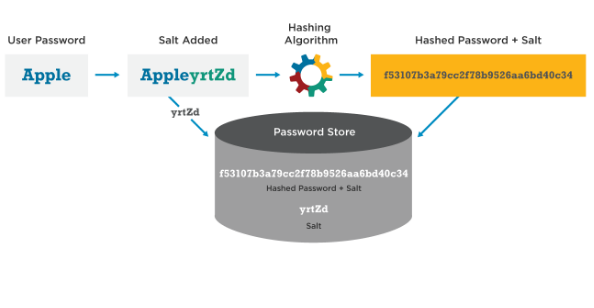
\includegraphics[scale=0.5]{images/prova.png}
        \caption{How salting works}
        \label{fig:salt}
    \end{figure}
    
    \FloatBarrier   
    
    As we can see salting is a good mitigation for the dictionary attacks.
    
    \subsection{Extension of password based authentication}
    We can extend the concept of passwords utilizing the multi factor authentication that can be performed by
    \begin{itemize}
        \item knowledge, something only the user knows (personal id number)
        \item ownership, something only the user possesses (token, smart card, phone)
        \item inherence, something the user is (biometrics)
    \end{itemize}
    The multi factor authentication is the combination of a password and another thing to perform the authentication (it can be also more than one another thing). The most common one is the 2FA (two factor authenticator), performed with a password and a OTP (one time password). Or a more common could be when you go to the ATM you insert the card and digit a PIN in order to use the services.
    
    \myparagraph{Time based One Time Password}
    OPT that has a deadline, they have two parameters the $T_0$ that is the Unix time from which start counting time steps, $T_x$ interval which will be used to calculate the value of the counter. Authenticator and authenticatee compute the TOTP value then the authenticator checks if the TOTP value supplied by the authenticated matches the locally-generated TOTP value. The weakness is that OTP values can be phished just as passwords can and replayed.
    \begin{figure}[h!]
        \centering
        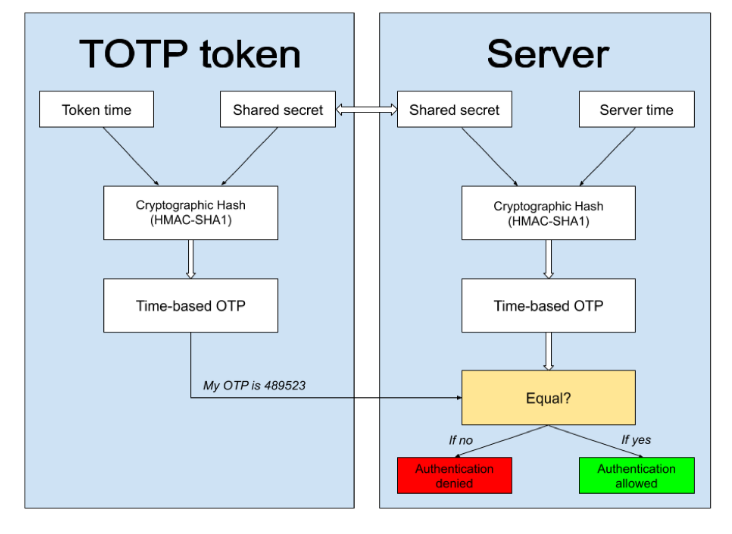
\includegraphics[scale=0.35]{images/TOTP.png}
        \caption{A TOTP communication}
        \label{fig:TOTP}
    \end{figure}
    
    \FloatBarrier   
    
    \myparagraph{Challenge Response Protocols}
    In CRP encryption convers the original representation of the information (\textbf{plaintext}) into an alternative form (ciphertext). Only authorized parties can decipher a ciphertext back to plaintext and access the original information. Encryption denies the intelligible content to a would-be interceptor.
    
    It's a mitigation for MITM attacks, since challenge changes at every connection, the MITM cannot reuse previously intercepted hashed password.
    
    \begin{figure}[h!]
        \centering
        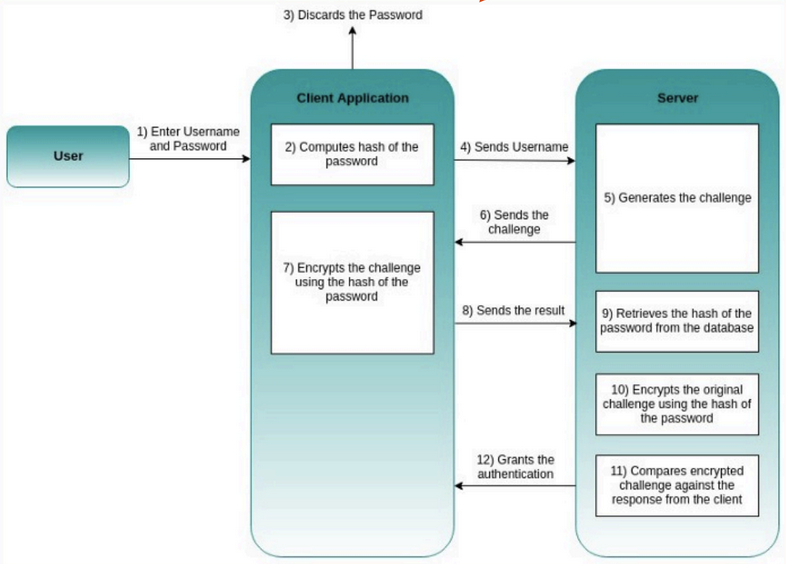
\includegraphics[scale=0.4]{images/CRP.png}
        \caption{CRP communication}
        \label{fig:CRP}
    \end{figure}
    
    \FloatBarrier   
    
    \myparagraph{PSD2}
    PSD2 is a solution to remove the TOTP hardware token, this because in the past they where hacked and they spoofed all the users. Chinese attackers spoofed Lockheed Martin staff-Sole plans for F-35 fighter jet. PSD2 idea is to include in the challenge the data that are unique to the particular transaction such as destination of transaction, amount of transaction ecc.
    
    We can also use \textbf{smartphones} as part of MFA, no additional token are required, dinamically generated passcodes are safer. It has it's disadvantages too, a mobile phone is not always available, the mobile connection is not always available, there are sim cloners, text message could be stolen.
    
    \myparagraph{Assurance level NIST}
    \begin{enumerate}
        \item Provides some assurance that the claimant controls the authenticator, require at least a \textbf{single factor authentication.}
        \item Provides high confidence that the claimant controls authenicators, \textbf{two different authentication factor} are required.
        \item Provides very high confidence that the claimant controls the authenticator, authentication based on \textbf{proof of possession of a key} through a cryptographic protocol.
    \end{enumerate}
    
    Unfortunately even MFA procedures can be vulnerable to phishing attacks, example MFA fatigue attacks.
    
    \myparagraph{FIDO}
    The main idea of fido is avoiding passwords, Google reported that it has not had any of it's 85000+ employees successfully phished on their work-related accounts since early 2017 when they started using physical security keys in place of passwords and one-time code.
    
    A security key implements a form of multi-factor authentication known as \textbf{Universal 2nd Factor (U2F)}, which allows the user to complete the login process simoly by inserting the USB device and pressing a button on it. Web Authentication API (\textbf{WebAuthn}) is a standard that eliminates the need for users to constantly type in their passwords and instead uses \textbf{Public key cryptography in combination with a challenge response protocol.} This avoid the possibility of phishing and MITM.
    
    FIDO requires an initial registration step: in cases where the user device supports multiple forms of authentication the user is asked to choose a FIDO compliant authenticator from the option available. The user then unlocks the FIDO authenticator using whatever mechanism is built into the authenticator, once is unlocked the user's device creates a new and unique public/private cryptographic key pair that will be used for authenticating access (\textbf{public one} is sent on the online server and associated with user account, the \textbf{private} and the other sensitive data remain on the local device and never leave it). Authentication requires the client device to prove possession of the private key by successfully respond to a cryptographic challenge. Private key can only be used after successfully authenticating using the registered authenticator, the device then uses the user account identifier provided by the service to select the correct key and cryptographically sign the service's challenge. Finally signed challenge is sent back to the service which verifies it and log in the user.
    
    \subsubsection{Outsourcing Authenticator}
    National digital identity infrastructures sponsored by many member states in europe obtained different level of success because of the not always clear business models for identity providers (an example of this is the Sistema Pubblico di Identità Digitale (SPID) in Italy. The problem is that securing all the phases of the identity management lifecycle is far from being trivial, organizations lack resources to devote ton security and need to focus on their core business. A solution could be to delegate the authentication to a trusted third party identity provider. Another example are the Single Sign On \textbf{(SSO)} like login with google or facebook ecc. This technique has lot of pros but a very big con: only one password to compose, if we use SSO+MFA we can improve a lot our security.